\documentclass[10pt,a4paper]{amsart}
\usepackage[utf8]{inputenc}
\usepackage[english]{babel}
\usepackage[mathcal]{euscript}
\usepackage{mathrsfs}  
\usepackage{amsmath}
\usepackage{amsfonts}
\usepackage{amssymb}
\usepackage{stmaryrd}
\usepackage{graphicx}
\usepackage{mathtools}
\usepackage{pgfplots}
\usepackage{xfrac}
\usepackage{listings}
\usepackage{xcolor}
\usepackage{lstlinebgrd}
\usepackage{ebproof}
\usepackage{graphicx,float}
\usepackage[colorlinks=true, linkcolor=cyan, urlcolor=cyan, citecolor=cyan]{hyperref}
\usepackage[shortlabels]{enumitem}
\usepackage[textsize=tiny,textwidth=45]{todonotes}

\newcommand{\klcomp}{\star}
\newcommand{\parI}{\mathop{\bowtie}}
\newcommand{\seqI}{\mathop{\triangleright}}
\DeclareMathOperator{\demon}{\square}
\DeclareMathOperator{\angel}{\Diamond}
\makeatletter
\DeclareRobustCommand{\iscircle}{\mathord{\mathpalette\is@circle\relax}}
\newcommand\is@circle[2]{%
  \begingroup
  \sbox\z@{\raisebox{\depth}{$\m@th#1\bigcirc$}}%
  \sbox\tw@{$#1\square$}%
  \resizebox{!}{\ht\tw@}{\usebox{\z@}}%
  \endgroup
}
\makeatother
\DeclareMathOperator{\statt}{\iscircle_\prog{p}}
\newcommand{\schfont}[1]{\mathcal{#1}}
\newcommand{\sch}{\schfont{S}}
\newcommand{\conv}[1]{\mathrm{conv}\, {#1}}
%%%%%%%%%%%%% Macros
\newcommand{\renato}[1]{\textcolor{teal}{RN Note: #1}}
\newcommand{\codiag}{\triangledown}
%%%% Categories
\newcommand{\catfont}[1]{\mathsf{#1}}
\newcommand{\cop}{\catfont{op}}
\newcommand{\Law}{\catfont{Law}}
\newcommand{\catV}{\catfont{V}}
\newcommand{\catX}{\catfont{X}}
\newcommand{\catC}{\catfont{C}}
\newcommand{\catCat}{\catfont{C}}
\newcommand{\catCop}{\catfont{C^{op}}}
\newcommand{\catD}{\catfont{D}}
\newcommand{\catE}{\catfont{E}}
\newcommand{\catA}{\catfont{A}}
\newcommand{\catB}{\catfont{B}}
\newcommand{\catP}{\catfont{P}}
\newcommand{\catMet}{\catfont{Met}}
\newcommand{\catCPTP}{\catfont{CPTP}}
\newcommand{\catCPS}{\catfont{CPS}}
\newcommand{\catCP}{\catfont{CP}}
\newcommand{\catQ}{\catfont{Q}}
\newcommand{\catSet}{\catfont{Set}}
\newcommand{\catFinSet}{\catfont{FinSet}}
\newcommand{\catPO}{\catfont{PO}}
\newcommand{\catCompFunc}{\catfont{CompFunc}}
\newcommand{\catBan}{\catfont{Ban}}
\newcommand{\catVect}{\catfont{CVect}}
\newcommand{\WstarCPSU}{\catfont{Wstar_{CPSU}}}
\newcommand{\WstarCPSUop}{\left(\catfont{Wstar_{CPSU}}\right)^{\catfont{op}}}
\newcommand{\catI}{\catfont{I}}
\newcommand{\Set}{\catfont{Set}}
\newcommand{\Top}{\catfont{Top}}
\newcommand{\Pos}{\catfont{Pos}}
\newcommand{\Inj}{\catfont{Inj}}
\newcommand{\Det}{\catfont{RMhat}}
\newcommand{\CoAlg}[1]{\catfont{CoAlg}\left (#1 \right )}
\newcommand{\Mon}{\catfont{Mon}}
\newcommand{\Mnd}{\catfont{Mnd}(\catC)}
\newcommand{\SMnd}{\catfont{Mnd}(\Set)}
\newcommand{\CLat}{\catfont{CLat}}
\newcommand{\SLat}{\catfont{SLat}}
\newcommand{\Stone}{\catfont{Stone}}
\newcommand{\Spectral}{\catfont{Spectral}}
\newcommand{\CompHaus}{\catfont{CompHaus}}
\newcommand{\Subs}[2]{\catfont{Sub}_{}}
\newcommand{\Cone}{\catfont{Cone}}
\newcommand{\LCone}{\catfont{LCone}}
\newcommand{\StComp}{\catfont{StablyComp}}
\newcommand{\PosC}{\catfont{PosComp}}
\newcommand{\Haus}{\catfont{Haus}}
\newcommand{\Meas}{\catfont{Meas}}
\newcommand{\Coh}{\catfont{CohDom}}
\newcommand{\Ord}{\catfont{Ord}}
\newcommand{\Dcpo}{\catfont{DCPO}}
\newcommand{\Dom}{\catfont{Dom}}
\newcommand{\EndoC}{[\catC,\catC]}
\newcommand{\Dcpop}{\catfont{DCPO}^\catfont{p}}
%% General functors
\newcommand{\funfont}[1]{#1}
\newcommand{\funF}{\funfont{F}}
\newcommand{\funU}{\funfont{U}}
\newcommand{\funG}{\funfont{G}}
\newcommand{\funT}{\funfont{T}}
\newcommand{\funI}{\funfont{I}}
%% Particular kinds of functors
\newcommand{\sfunfont}[1]{\mathrm{#1}}
\newcommand{\Pow}{\sfunfont{P}}
\newcommand{\PP}{\sfunfont{V}}
\newcommand{\Dist}{\sfunfont{V}_{=1,\omega}}
\newcommand{\PDist}{\sfunfont{V}_{\leq 1,\omega}}
\newcommand{\Maybe}{\sfunfont{M}}
\newcommand{\List}{\sfunfont{L}}
\newcommand{\UForg}{\sfunfont{U}}
\newcommand{\Forg}[1]{\sfunfont{U}_{#1}}
\newcommand{\Id}{\sfunfont{Id}}
\newcommand{\Vie}{\sfunfont{V}}
\newcommand{\Disc}{\funfont{D}}
\newcommand{\Weight}{\sfunfont{W}}
\newcommand{\homf}{\sfunfont{hom}}
\newcommand{\Yoneda}{\sfunfont{Y}}
%% Diagram functors
\newcommand{\Diag}{\mathscr{D}}
\newcommand{\KDiag}{\mathscr{K}}
\newcommand{\LDiag}{\mathscr{L}}
%% Monads
\newcommand{\monadfont}[1]{\mathbb{#1}}
\newcommand{\monadT}{\monadfont{T}}
\newcommand{\monadS}{\monadfont{S}}
\newcommand{\monadU}{\monadfont{U}}
\newcommand{\monadH}{\monadfont{H}}
\newcommand{\str}{\mathrm{str}}
%% Adjunctions
\newcommand\adjunct[2]{\xymatrix@=8ex{\ar@{}[r]|{\top}\ar@<1mm>@/^2mm/[r]^{{#2}}
& \ar@<1mm>@/^2mm/[l]^{{#1}}}}
\newcommand\adjunctop[2]{\xymatrix@=8ex{\ar@{}[r]|{\bot}\ar@<1mm>@/^2mm/[r]^{{#2}}
& \ar@<1mm>@/^2mm/[l]^{{#1}}}}
%% Retractions
\newcommand\retract[2]{\xymatrix@=8ex{\ar@{}[r]|{}\ar@<1mm>@/^2mm/@{^{(}->}[r]^{{#2}}
& \ar@<1mm>@/^2mm/@{->>}[l]^{{#1}}}}
%% Limits
\newcommand{\pv}[2]{\langle #1, #2 \rangle}
\newcommand{\limt}{\mathrm{lim}}
\newcommand{\pullbackcorner}[1][dr]{\save*!/#1+1.2pc/#1:(1,-1)@^{|-}\restore}
\newcommand{\pushoutcorner}[1][dr]{\save*!/#1-1.2pc/#1:(-1,1)@^{|-}\restore}
%% Colimits
\newcommand{\colim}{\mathrm{colim}}
\newcommand{\inl}{\mathrm{inl}}
\newcommand{\inr}{\mathrm{inr}}
%% Distributive categories
\newcommand{\distr}{\mathrm{dist}}
\newcommand{\undistr}{\mathrm{undist}}
%% Closedness
\newcommand{\curry}[1]{\mathrm{curry}{#1}}
\newcommand{\app}{\mathrm{app}}
%% Misc. operations
\newcommand{\const}[1]{\underline{#1}}
\newcommand{\comp}{\cdot}
\newcommand{\id}{\mathrm{id}}
\newcommand{\sw}{\mathrm{sw}}
\newcommand{\spt}{\mathrm{sp}}
\newcommand{\sh}{\mathrm{sh}}
\newcommand{\jn}{\mathrm{jn}}
\newcommand{\dist}{\mathrm{dist}}
\newcommand{\unfold}{\mathrm{unfold}}
\newcommand{\fold}{\mathrm{fold}}
%% Factorisations
\newcommand{\EClass}{E}
\newcommand{\MClass}{M}
\newcommand{\MConeClass}{\mathcal{M}}
%%%%%%%%%%%%%%%% End of Categorical Stuff

%%%% Misc
%% Operations
\newcommand{\blank}{\, - \,}
\newcommand{\sem}[1]{\left \llbracket #1 \right \rrbracket}
\newcommand{\asem}[1]{ \llparenthesis #1 \rrparenthesis}
\newcommand{\closure}[1]{\overline{#1}}
\DeclareMathOperator{\img}{\mathrm{im}}
\DeclareMathOperator{\dom}{\mathrm{dom}}
\DeclareMathOperator{\codom}{\mathrm{codom}}
%% Sets of numbers
\newcommand{\Nats}{\mathbb{N}}
\newcommand{\Reals}{\mathbb{R}}
\newcommand{\Rats}{\mathbb{Q}}
\newcommand{\Rz}{\Reals_{\geq 0}}
\newcommand{\Complex}{\mathbb{C}}
%% Writing
\newcommand{\cf}{\emph{cf.}}
\newcommand{\ie}{\emph{i.e.}}
\newcommand{\eg}{\emph{e.g.}}
\newcommand{\df}[1]{\emph{\textbf{#1}}}
%%%%%%%%%%%%%%%% End of Misc

%%%% Programming Stuff
%% Types
\newcommand{\typefont}[1]{\mathbb{#1}}
\newcommand{\typeOne}{1}
\newcommand{\typeTwo}{2}
\newcommand{\typeA}{\typefont{A}}
\newcommand{\typeB}{\typefont{B}}
\newcommand{\typeC}{\typefont{C}}
\newcommand{\typeV}{\typefont{V}}
\newcommand{\typeD}{\typefont{D}}
\newcommand{\typeE}{\typefont{E}}
\newcommand{\typeF}{\typefont{F}}
\newcommand{\typeI}{\typefont{I}}
%% RuleName
\newcommand{\rulename}[1]{(\mathrm{#1})}
%% Sequents
\newcommand{\jud}{\vdash}
\newcommand{\vljud}{\triangleright}
\newcommand{\cojud}{\vdash_{\co}}
\newcommand{\vl}{\mathtt{v}}
\newcommand{\co}{\mathtt{c}}
% Program font
\newcommand{\prog}[1]{\ensuremath{\tt #1}}
\newcommand{\blue}[1]{\textcolor{blue}{#1}}
\newcommand{\pseq}[3]{#1 \leftarrow #2; #3}
\newcommand{\ppm}[4]{(#1,#2) \leftarrow #3; #4}
\newcommand{\pinl}[1]{\prog{inl}(#1)}
\newcommand{\pinr}[1]{\prog{inr}(#1)}
\newcommand{\pcase}[5]{\prog{ case } #1 \prog{ \hspace{2pt} of \hspace{2pt} } \pinl{#2} \Rightarrow #3 ; \pinr{#4} \Rightarrow #5}
%% Sets of terms
\newcommand{\ValuesBP}[2]{\mathsf{Values}(#1, #2)}
\newcommand{\TermsBP}[2]{\mathsf{Terms}(#1, #2)}
\newcommand{\closValP}[1]{\ValuesBP{\emptyset}{#1}}
\newcommand{\closTermP}[1]{\TermsBP{\emptyset}{#1}}
\newcommand{\closVal}{\closValP{\typeA}}
\newcommand{\closTerm}{\closTermP{\typeA}}
%% Contextual equivalence
\newcommand{\ctxeq}{\equiv_{\prog{ctx}}}

%%%% End of Programming Stuff
\newcommand{\Shuff}{\mathrm{Sf}}

%%%% Domain theory
\newcommand{\upclos}{\mathord{\uparrow}}
\newcommand{\dwclos}{\mathord{\downarrow}}

%%%% Quantum stuff
\newcommand{\Hilb}{\catfont{Hilb}}
\newcommand{\tr}{\text{Tr}}

%%%% Norms
\newcommand{\euclideannorm}[1]{\left\lVert #1  \right\rVert_{2}}
\newcommand{\spectralnorm}[1]{\left\lVert #1  \right\rVert_{\infty}}
\newcommand{\tracenorm}[1]{\left\lVert #1  \right\rVert_{1}}
\newcommand{\diamondnorm}[1]{\left\lVert #1  \right\rVert_{\diamondsuit}}
\newcommand{\lonenorm}[1]{\left\lVert #1  \right\rVert_{ L^{1} }}
\newcommand{\gentracenorm}[1]{\left\lVert #1  \right\rVert_{ L^\infty }}
\newcommand{\gendiamondnorm}[1]{\left\lVert #1  \right\rVert_{ \diamondsuit \text{ gen}}}
\newcommand{\opnorm}[1]{\left\lVert #1  \right\rVert_{\text{op}}}
\newcommand{\norm}[1]{\left\lVert #1  \right\rVert}
\newcommand{\cbnorm}[1]{\left\lVert #1  \right\rVert_{\text{cb}}}
\newcommand{\projnorm}[1]{\left\lVert #1  \right\rVert_{\pi}}

%%%% Tensor
\newcommand{\projtensor}{\widehat{\otimes}_\pi}

\usepackage[left=2cm,right=2cm,top=2cm,bottom=2cm]{geometry}
\usepackage{tcolorbox}
\usepackage{braket}
\usepackage{quantikz}
\usepackage{tikz-cd}
\linespread{1.10}
\author{\dots}
\title{Notes}

\lstset{
language=C,
showstringspaces=false,
keywordstyle=\color{blue},
basicstyle=\fontsize{10}{13}\ttfamily,
emph={exit,blue,unif,then,wait},emphstyle=\color{blue},
breaklines=true,
escapeinside={*@}{*@}
}


\usepackage{proof}
\usepackage{amsthm}
\usepackage[all]{xy}
%for definition
\theoremstyle{definition}
\newtheorem{definition}{Definition}[section]

%for examples
\theoremstyle{definition}
\newtheorem{example}[definition]{Example}

%lemmas
\theoremstyle{definition}
\newtheorem{lemma}[definition]{Lemma}

%proposition
\theoremstyle{definition}
\newtheorem{proposition}[definition]{Proposition}
%corollary
\theoremstyle{definition}
\newtheorem{corollary}[definition]{Corollary}

%theorem
\theoremstyle{definition}
\newtheorem{theorem}[definition]{Theorem}

% Renato's macros
\newcommand{\until}{\> \textcolor{blue}{\prog{for}} \>}
\newcommand{\then}{\textcolor{blue}{then}}
\newcommand{\progife}[3]{{ \blue{\prog{if}} \> #1 \> \blue{\prog{then}} \> 
{\prog #2} \> \blue{\prog{else}} \> {\prog #3}}}
\newcommand{\progwhile}[2]{{\blue{\prog{while}} \>  #1 \> \blue{\prog{do}} \> \{ \> {#2}  \> \}}}
\newcommand{\scomp}{\, \blue{;} \,}
\newcommand{\prem}[1]{(\text{if\/ }#1)}
\newcommand{\nline}{\vspace{-5mm}}
\newcommand{\ssto}[1][]{~\to^{#1}~}
\newcommand{\bsto}{~\Downarrow~}
\newcommand{\stp}{\mathit{stop}}
\newcommand{\skp}{\mathit{skip}}
\newcommand{\err}{\mathit{err}}
\providecommand{\comma}{,\operatorname{}\linebreak[1]}		% possibly line-beaking comma
\newcommand{\sep}{\kern1pt\comma\kern-1pt}
\newcommand{\lrule}[3]{\textbf{#1}\quad\frac{#2}{#3}}
\newcommand{\ptt}{{\prog tt}}
\newcommand{\pff}{{\prog ff}}
\newcommand{\unif}{{\prog \blue{unif}}}
\newcommand{\meas}[1]{\mathcal{M}(#1)}
\newcommand{\pmap}{ \xrightharpoonup{\hspace{0.1cm}} }

\begin{document}
\title{Quantum stuff}
\maketitle
%\tableofcontents
\section{Lambda-calculus with conditionals}

\subsection{Syntax}

Considering a class $G$ of ground types, the grammar of types for linear lambda calculus with conditionals corresponds to:

\begin{equation*} \label{eq:grammartypes}
  \centering
   \mathbb{A} ::= X \in G \hspace{3 pt} \vert \hspace{3 pt} \mathbb{I}  \hspace{3 pt}  \vert \hspace{3 pt} \mathbb{A}  \otimes  \mathbb{A} \hspace{3 pt} \vert  \hspace{3 pt} \mathbb{A}  \oplus \mathbb{A} \hspace{3 pt}  \vert  \hspace{3 pt} \mathbb{A} \multimap  \mathbb{A}
  \end{equation*}

The term formation rules for conditionals are depicted in \autoref{fig:typing_rules_cond}. 

\begin{figure}[H]
    \begin{equation*}
    \begin{aligned}
    &\hspace{10pt}
    %
    \begin{prooftree}
        \hypo{\Gamma \vljud v: \typeA}
        \infer1[(inl)]{\Gamma \vljud \inl_{\typeB}(v): \typeA \oplus \typeB}
    \end{prooftree}
    %
    \hspace{30pt}
    %
    \begin{prooftree}
        \hypo{\Gamma \vljud v: \typeB}
        \infer1[(inr)]{\Gamma \vljud \inr_{\typeA}(v): \typeA \oplus \typeB}
    \end{prooftree} 
    %
    \\[20pt]
    &\hspace{-20pt}
    %
    \begin{prooftree}
        \hypo{\Gamma \vljud v: \typeA \oplus \typeB}
        \hypo{\Delta, x: \typeA \vljud w: \typeD}
        \hypo{\Delta, y: \typeB \vljud u: \typeD}
        \hypo{E \in \Shuff(\Gamma; \Delta)}
        \infer4[(case)]{E \vljud \text{case } v\,
        \{\inl_{\typeB}(x) 
            \Rightarrow w ; \,
          \inr_{\typeA}(y) \Rightarrow u
        \}: \typeD}
    \end{prooftree}
    %
    \\[10pt]
    \end{aligned}
    \end{equation*}
    \caption{Term formation rules for conditionals}
    \label{fig:typing_rules_cond}
\end{figure}
The rules presented in Figure \ref{fig:typing_rules_cond} enjoy the following
properties.

\begin{theorem} \label {theorem:unique_der}
   Lambda calculus with conditionals has the following properties:
   \begin{enumerate}
     \item\label{perm} for all judgements $\Gamma \vljud v$ and $\Gamma'
             \vljud v$, te($\Gamma$) $\simeq_{\pi}$  te($\Gamma'$); 
     %
     \item\label{type} additionally if $\Gamma \vljud v: \typeA,
       \Gamma' \vljud v: \typeA'$, and $\Gamma \simeq_{\pi}
       \Gamma'$, then $\typeA$ must be equal to $\typeA'$;
     %
     \item\label{der} all judgements $\Gamma \vljud v:\typeA$ have a unique derivation.
\end{enumerate}
\end{theorem}
%
\begin{proof}
It follows in all three cases from induction over the length of derivation
trees. 

Let us focus first on Property~\eqref{perm}. The case of the rules concerning
injections is direct. As for rule~$\rulename{cond}$ take two contexts $E$ and
$E'$ for the same conditional. According to this rule we obtain contexts
$\Gamma$, $\Gamma'$, $\Delta$, $\Delta'$ such that $E \in
\Shuff(\Gamma;\Delta)$ and $E' \in \Shuff(\Gamma';\Delta')$. It follows from
induction that  $\Gamma \simeq_\pi \Gamma'$ and $\Delta \simeq_\pi \Delta'$,
and the proof is then obtained from the sequence of equivalences,
\begin{align*}
        \text{te}(E) & \simeq_\pi \text{te}(\Gamma, \Delta) 
        \\
        & \simeq_\pi \text{te}(\Gamma', \Delta')
        \\
        & \simeq_\pi \text{te}(E')
\end{align*}
Concerning Property~\eqref{type}, the case of the rules concerning injections
is direct and the case of rule~$\rulename{cond}$ is a corollary of
Property~\eqref{perm}. Finally let us consider Property~\eqref{der}. Again the
case concerning injections is direct and we thus focus only on
rule~$\rulename{cond}$. According to this rule we obtain contexts $\Gamma$,
$\Gamma'$, $\Delta$, $\Delta'$ such that $E \in \Shuff(\Gamma;\Delta)$ and $E
\in \Shuff(\Gamma';\Delta')$. By an appeal to Property~\eqref{perm} we also
obtain $\Gamma \simeq_\pi \Gamma'$ and $\Delta \simeq_\pi \Delta'$, and thus
since shuffling preserves relative orders we obtain $\Gamma = \Gamma'$ and
$\Delta = \Delta'$. The proof then follows by induction.
\end{proof}

\begin{lemma}[Exchange and Subsitution]
\label{exh_and_sub} 
For every judgement $\Gamma,x: \typeA, y: \typeB, \Delta \vljud v: \typeD$ the
judgement $\Gamma, y:\mathbb{B}, x:\mathbb{A}, \Delta \vljud v:
\typeD$ is derivable. Not only this, given judgements  $\Gamma,x:\typeA \vljud
v: \typeB$ and $\Delta \vljud w: \typeA$ the judgement $\Gamma, \Delta \vljud
v[w/x]: \typeB$ is also derivable.
\end{lemma}

\begin{proof}
We start with the exchange property which follows by induction over the length
of derivation trees. The rules that involve injections are direct.  The rule
$\rulename{case}$ calls for case distinction, more specifically we  distinguish
between the cases in which both variables ($x : \typeA$ and $y : \typeB$) are
in $\Gamma$, both are in $\Delta$, and otherwise. The first two cases follow
straightforwardly by induction and the definition of a shuffle. For the third
case consider a judgement $E_1,x : \typeA, y : \typeB, E_2 \vljud \text{case }
v\, \{\inl_{\typeF}(a) \Rightarrow w ; \, \inr_{\typeE}(b) \Rightarrow u \}:
\typeD$, and assume with no loss of generality that $\Gamma$ is of the form
$\Gamma_1, x : \typeA, \Gamma_2$ and $\Delta$ of the form $\Delta_1, y :
\typeB, \Delta_2$. The proof now follows directly from the implication,
\[
        E_1, x : \typeA, y : \typeB, E_2 \in \Shuff(\Gamma_1, x : \typeA, \Gamma_2 ; \,
        \Delta_1, y : \typeB, \Delta_2)
        \Longrightarrow
        E_1, y : \typeB, x : \typeA, E_2 \in \Shuff(\Gamma_1, x : \typeA, \Gamma_2 ; \,
        \Delta_1, y : \typeB, \Delta_2)
\]
(which holds by the definition of a shuffle).

Finally we now focus on the substitution rule which also follows by induction over the
length of derivation trees. Again the cases involving the injections are direct,
and we thus only detail the proof of rule $\rulename{case}$. Consider then
judgements $E,x : \typeA \vljud \text{case } v\, \{\inl_{\typeD}(a) \Rightarrow
w ; \, \inr_{\typeE}(b) \Rightarrow u \}: \typeB$ and
$Z \vljud t : \typeA$ with $E \in \Shuff(\Gamma; \Delta)$. According to the definition
of a shuffle either $\Gamma$ is of the form $\Gamma_1, x: \typeA$ or $\Delta$ is
of the form $\Delta_1, x : \typeA$. The first case follows directly and the second case
is a corollary of the exchange rule.
\end{proof}
 
The equational system for the conditionals is shown in Figure
\ref{fig:equations-in-context-cond}.


  \begin{figure}[h!]
    \centering
    \begin{tcolorbox}[colframe=black, colback=white, boxrule=0.6pt, arc=1pt,boxsep=1pt,top=1pt,bottom=1pt, width=0.85 \textwidth]
    \begin{equation*}
        \begin{split}
          &(\beta_{case}^{inl}) \hspace{3pt} \text{ case } 
          \inl_{\typeB}(v) \hspace{2pt} \{ \inl_{\typeB} (x) \Rightarrow w 
          ; \hspace{1pt} \inr_{\typeA} (y) 
          \Rightarrow u\}= w[v/x]
          %
          \\
          %
          &(\beta_{case}^{inr}) \hspace{3pt} \text{ case } 
          \inr_{\typeA}(v) \hspace{2pt} \{ \inl_{\typeB} (x) \Rightarrow w 
          ; \hspace{1pt} \inr_{\typeA} (y) 
          \Rightarrow u\}= u[v/y]
          %
          \\
          %
          %
          & (\eta_{case}) \hspace{3pt} \text{ case }(v)\ \hspace{2pt} \{\text{inl}_{\mathbb{B}} (y) \Rightarrow w [ \text{inl}_{\mathbb{B}}(y)/x] ; \hspace{1pt} \text{inr}_{\mathbb{A}} (z) \Rightarrow w [ \text{inr}_{\mathbb{A}}(z)/x]\} = w[v/x] : \mathbb{D}
        \end{split}
    \end{equation*}
    \end{tcolorbox}
    \caption{Equational system for the conditionals}
    \label{fig:equations-in-context-cond}
    \end{figure}


    \subsubsection{Examples of Programs (Quantum Setting)}

    \par\vspace{10pt} 
    
    
    In the case of quantum lambda calculus, it is natural to consider a  type $\textit{qbit}$ of quantum bits and a type $\textit{bit}$ of classical bits.  The following operations are considered: the creation of a new bit $(1,0)$, $\textit{new} \hspace{2pt} 0  :\mathbb{I}  \multimap \textit{bit} $, the creation of a new bit $(0,1)$, $\textit{new} \hspace{2pt} 1  :\mathbb{I}  \multimap \textit{bit} $, the conversion of a bit into a qubit, $q : \textit{bit}  \multimap \textit{qbit}$, measuring a qubit, $\textit{meas}:\textit{qbit} \xrightarrow{} \textit{bit}$, applying a unitary  operation to a qubit $\textit{U}:\textit{qbit},\ldots,\textit{qbit} \xrightarrow{} \textit{qbit}^{\otimes n}$, and performing a CPTP operation on a qubit, $\textit{CPTP}: \textit{qbit}^{\otimes n} \multimap \textit{qbit}^{\otimes n}$. 


    \textbf{Quantum State Discrimination}


Quantum state discrimination is a pivotal challenge in quantum information, fundamental to the extraction of classical information from quantum systems. While orthogonal states can be perfectly distinguished, the same does not apply to nonorthogonal states. 
Even when the set of possible nonorthogonal states is known, determining the optimal discrimination strategy is considered a nontrivial problem.

For example, when distinguishing between two nonorthogonal quantum states, the Helstrom measurement represents the optimal strategy \cite{helstromQuantumDetectionEstimation1976}. In the case where both states are pure, the Helstrom measurement corresponds to a projective measurement \cite{barnett2009quantum}.

When operating within the computational basis, a projective measurement can be understood as the application of a unitary operator, followed by a subsequent measurement in the computational basis. In this context, the Helstrom measurement can be interpreted as a unitary transformation applied to the quantum state, followed by a measurement in the computational basis. 

Consider the task of discriminating between two pure states $\ket{\psi_0}$ and $\ket{\psi_1}$, prepared with a priori probabilities $p_0$ and $p_1$, respectively. Let the unitary operator $U$  be the transformation that rotates the computational basis to the basis associated with the Helstrom measurement  in this context. This discrimination task can then be formalized as follows:

\begin{align*}
  &\textbf{StatePreparation} =  b:\textit{bit}  \triangleright  \text{case } b \{\text{inl}_{\mathbb{B}}(x) \Rightarrow \ket{\psi_0} ; \text{inr}_{\mathbb{A}}(y) \Rightarrow \ket{\psi_1}\}: \textit{qbit} \\
  &\textbf{HMeasure} =  q_0: \textit{qbit} \triangleright \textit{meas} (\textit{U}(q_0))  : \textit{qbit} \\
  &\textbf{Discrimination} = (p_0,p_1): \textit{bit}  \triangleright \textbf{HMeasure} [ \textbf{StatePreparation} [(p_0,p_1)/ b] / q_0] : \textit{bit}
\end{align*}



\vspace{10pt}



    \textbf{ Quantum Teleportation}


    \cite{bennett1993teleporting} introduced the concept of quantum teleportation, which is a protocol that allows the transfer of   unknown quantum states between distant parties.  The quantum teleportation protocol is a fundamental building block for quantum communication, quantum computation, and quantum networks, its applications ranging
from secure quantum communication to distributed quantum computing \cite{briegel1998quantum,gottesman1999demonstrating,kimble2008quantum}.

Conceptually the protocol can be described as follows: Alice and Bob share an entangled pair of qubits, which are in a Bell state. Alice keeps the first qubit and Bob the second. Moreover, Alice has a qubit in an unknown state $\ket{\psi}$ that she wants to send to Bob.  
 Alice entangles her qubit and the firt qubit of the Bell state, and then measures them. The result of this measurement is two classical bits that Alice sends to Bob though a classical channel. Based on the measurement results, Bob applies a correction to his qubit so it matches the initial state $\ket{\psi}$. 
The circuit corresponding to the implementation of the quantum teleportation protocol is depicted in \autoref{fig:teleport}.


\begin{figure} [H]
  \centering
  \begin{quantikz} [column sep=0.2cm, row sep=0.5cm] 
      \lstick{$\ket{\psi}$}  & \qw &\qw & \qw & \qw & \qw& \ctrl{1}\gategroup[2,steps=4,style={dashed,rounded
      corners,fill=blue!20, inner
      xsep=2pt},background,label style={label
      position=below,anchor=north,yshift=-0.2cm}]{{\sc
      BellMeasure}} & \gate{H} & \qw & \meter{} & \setwiretype{c}  &  & \gategroup[3,steps=4,style={dashed,rounded
      corners,fill=blue!20, inner
      xsep=2pt},background,label style={label
      position=below,anchor=north,yshift=-0.2cm}]{{\sc
      Correction}}  &  & & \ctrl[vertical
wire=c]{2}  \\
      \lstick {$\ket{0}$}  &\gate{H}\gategroup[2,steps=3,style={dashed,rounded
      corners,fill=blue!20, inner
      xsep=2pt},background,label style={label
      position=below,anchor=north,yshift=-0.2cm}]{{\sc
      EPR}} & \qw  & \ctrl{1}& \qw & \qw & \targ{} & \qw & \qw & \meter{} & \setwiretype{c} & & & \ctrl[vertical
wire=c]{1} \\
      \lstick{$\ket{0}$}  &  \qw & \qw &  \targ{} & \qw &\qw&\qw & \qw & \qw& \qw & \qw & \qw &  \qw & \gate{X} & \qw & \gate{Z} 
 \end{quantikz}
  \caption{Quantum Teleportation Protocol}
  \label{fig:teleport}
\end{figure}

When formalizing the quantum teleportation protocol within the lambda calculus framework, each part of the protocol is instantiated as a distinct function. 
Considering the unitary operations $H: \textit{qbit} \multimap  \textit{qbit}$, $X: \textit{qbit} \multimap  \textit{qbit}$, $Z: \textit{qbit} \multimap  \textit{qbit}$, $I: \textit{qbit} \multimap  \textit{qbit}$, and $\textit{CNOT}: \textit{qbit}, \textit{qbit} \multimap  \textit{qbit} \otimes \textit{qbit}$ , these functions are defined as follows:

\begin{align*}
   &\textbf{EPR} =  - \triangleright  \textit{CNOT} \hspace{2pt} (\textit{H}\hspace{2pt} (q  \hspace{2pt}    ( \textit{new}   \hspace{2pt}  0 \hspace{1pt}(*))),(q  \hspace{2pt}   ( \textit{new}   \hspace{2pt}  0 \hspace{1pt}(*)))) : \textit{qbit} \otimes \textit{qbit}  \\ 
      &\textbf{BellMeasure} =  q_{1}: \textit{qbit}, q_{2}: \textit{qbit}  \triangleright  \text{pm}  \hspace{2pt} \textit{CNOT} (q_{1},q_{2})  \hspace{2pt}  \text{to} \hspace{2pt} x \otimes y.  \hspace{2pt}  \textit{meas} (\textit{H} (x)) \otimes \textit{meas} (y) :  \textit{bit} \otimes \textit{bit} \\
      &\textbf{Correction}= q: \textit{qbit}, x: \text{bit},  y: \text{bit} \triangleright  \text{case } x  \hspace{2pt}  \{\text{inl} (x_{0}) \Rightarrow  \text{case}\hspace{2pt} y  \hspace{2pt}  \{\text{inl} (y_{0})  \Rightarrow{}  \textit{I}(q); \\
      & \hspace{275pt} \text{inr} (y_{1}) \Rightarrow  \hspace{2pt}   \textit{X} (q)\} ; \\
      & \hspace{200pt}\text{inr} (x_{1})  \Rightarrow  \text{case}\hspace{2pt} y  \hspace{2pt}  \{\text{inl} (y_{0})  \Rightarrow   \textit{Z}(q);  \\
      &\hspace{275pt} \text{inr} (y_{1}) \Rightarrow{} \textit{Z} (\textit{X}(q)) \}\} : \textit{qbit}
 \end{align*}


 Designating the qubit to be teleported as $qb_0$, one can conceptualize the teleportation procedure as follows:
 \begin{align*}
  \textbf{QTP} = qb_{0}: \textit{qbit}\hspace{3 pt} \triangleright \hspace{3 pt} & \text{pm} \hspace{5pt} \textbf{EPR} \hspace{5pt} \text{to} \hspace{5pt}  qb_{1} \otimes qb_{2}.  \notag \\
     & \text{pm}\hspace{5pt} \textbf{BellMeasure} \hspace{1pt} [qb_0/q_1,qb_{1}/q_2] \hspace{5pt}  \text{to} \hspace{5pt} c_{0}\otimes c_{1} . \notag \\
     & \text{pm} \hspace{5pt}  \textbf{Correction} \hspace{1pt} [qb_{2}/q,c_{0}/x, c_{1}/y]  \hspace{5pt} \text{to} \hspace{5pt}  qb. \hspace{2pt}  qb : \textit{qbit} 
 \end{align*}

 
 \subsection{Interpretation}

With the syntax of conditionals in lambda calculus established, it is now essential to define the meaning of the calculus's terms within the ``reality'' of interest—that is, to provide an interpretation for the calculus's conditionals, also known as the model of this ``reality''. In this work, the model is based on monoidal closed categories with coproducts. 

A monoidal category is a category equipped with a bifunctor $\otimes: \mathcal{C} \times \mathcal{C} \xrightarrow{} \mathcal{C}$, an object $I$, and natural isomorphisms $\alpha: (A \otimes B) \otimes C \xrightarrow{} A \otimes (B \otimes C)$, $\lambda: I \otimes A \xrightarrow{} A$, and $\rho: A \otimes I \xrightarrow{} A$ that satisfy the pentagon and triangle identities. A monoidal category $\mathcal{C}$ is monoidal closed if, for each object $A$ in $\mathcal{C}$, the functor $A \otimes - : \mathcal{C} \to \mathcal{C}$ has a right adjoint, denoted by $A \multimap -$. %This is equivalent to the existence of an internal hom bifunctor $\multimap : \mathcal{C}^{op} \times \mathcal{C} \to \mathcal{C}$, together with a natural isomorphism $\text{ev}_{A,B} : (A \multimap B) \otimes A \to B$.  
\todo[inline,size=\normalsize]{Pelo que eu percebi normalmente quando se fala de category monoidal fechada usa-se o funtor $- \otimes A$ ao invés de $A \otimes -$, mas eu defini assim dado como a distribuição do tensor sobre o coproduto tem de ser definida abaixo.} 
Considering a category $\mathcal{C}$  with objects $A$ and $B$, a coproduct of $A$ and $B$ is an object $A \oplus B$ with injection morphisms $i_A$ and $i_B$. Additionally, these satisfy the following universal property: for every object $C$ and any two maps $f $ and $g$, there exists a unique map $[f,g] : A \oplus B \rightarrow C$ which makes both triangles commute.

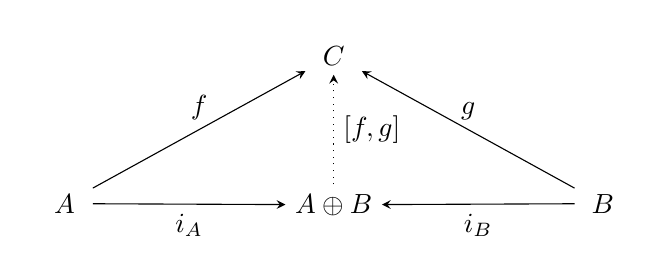
\begin{tikzpicture}
  \matrix (m) [matrix of math nodes,row sep=4em,column sep=7em,minimum width=2em]
  {
   & C &  \\
    A  & A \oplus B & B\\
  };
  \path[-stealth]
    (m-2-1) edge  node [above] {$f$} (m-1-2)
    (m-2-3) edge  node [above] {$g$} (m-1-2)
    (m-2-1) edge  node [below] {$i_A$} (m-2-2)
    (m-2-3) edge  node [below] {$i_B$} (m-2-2)
    (m-2-2) edge [dotted]  node [right] {$[f,g]$} (m-1-2);
    ;
\end{tikzpicture}

A few examples of monoidal closed categories with coproducts include the category of sets, the category of vector spaces, and the category of partial orders.
\todo[inline,size=\normalsize]{Explicar melhor em que consiste cada categoria? (o que são os objetos e morfismos)} 



To interpret the conditionals, it is first necessary to establish some notation. Let $\mathcal{C}$ be a monoidal closed category and let $X,$ $Y,$ and $Z$ be objects in $\mathcal{C}$. The morphism $\text{dist}_{X, Y,Z}: X \otimes  \left(Y \oplus Z\right) \xrightarrow{} \left(X \otimes Y\right) \oplus \left(X \otimes Y\right)$, denotes the distributive property of the tensor product over the coproduct.  This distributive property holds in monoidal closed categories with coproducts because the tensor functor is a left adjoint (to the internal hom), and left adjoints preserve colimits.
The type $A \oplus B$ is interpreted as $[\![A \oplus B ]\!] = [\![A ]\!] \oplus [\![ B ]\!]$. The interpretation of conditionals is illustrated in \autoref{fig:denotational_sem cond}.

\begin{figure}[H]
  \begin{equation*}
  \begin{aligned}
  &\hspace{10pt}
  %
  \begin{prooftree}
      \hypo{ [\![\Gamma \triangleright v: \mathbb{A}]\!] = m }
      \infer1[]{ [\![ \Gamma \triangleright \text{inl} (v):  \mathbb{A} \oplus \mathbb{B}  ]\!] = i_{\mathbb{A}}  \cdot m}
  \end{prooftree}
  %
  \hspace{30pt}
  %
  \begin{prooftree}
    \hypo{ [\![\Gamma \triangleright v: \mathbb{B}]\!] = m }
    \infer1[]{ [\![ \Gamma \triangleright \text{inl} (v):  \mathbb{B} \oplus \mathbb{B}  ]\!] = i_{\mathbb{B}}  \cdot m}
\end{prooftree}
  %
  \\[20pt]
  &\hspace{-20pt}
  %
  \begin{prooftree}
      \hypo{[\![\Gamma\triangleright v: \mathbb{A} \oplus \mathbb{B} ]\!] = b}
      \hypo{[\![\Delta, x:\mathbb{A} \triangleright w: \mathbb{D} ]\!] = p}
      \hypo{ [\![\Delta,y:\mathbb{B} \triangleright u: \mathbb{D} ]\!] = q }
      \hypo{E \in \Shuff(\Gamma; \Delta)}
      \infer4[]{ [\![E \triangleright \text{ case } v \hspace{2pt}  \{\text{inl} (x) \Rightarrow w ; \hspace{1pt} \text{inr} (y) \Rightarrow u\}: \mathbb{D} ]\!] =   [p \cdot \text{jn}_{\Delta;\mathbb{A}},q \cdot \text{jn}_{\Delta;\mathbb{B}}] \cdot \text{dist} \cdot \text{sw} \cdot (b \otimes \text{id}) \cdot \text{sp}_{\Gamma;\Delta} \cdot \text{sh}_{E}}
  \end{prooftree}
  %
  \\[10pt]
  \end{aligned}
  \end{equation*}
  \caption{Judgment interpretation for conditionals}
\label{fig:denotational_sem cond}
\end{figure}






%\todo[inline,size=\normalsize]{Elitzur‑Vaidman Bomb Testing Problem -> Improve usando o efeito Zeno? -> Acho que não tem ifs} 

\bibliographystyle{alpha} 
\bibliography{biblio}
\end{document}
